A commonn method of analyzing dynamical systems is plotting a trajectory's return to a Poincar\'e section. In some cases one can also use it to prove the existence of a limit cycle or chaotic behavior. When it comes to visualization, one can only plot a handful of different trajectories in a Poincar\'e section before the image becomes too busy and illegible, so we see the details of a selection of trajectories and not the full picture.

We propose to apply a similar procedure for Poincar\'e sections as in the previous section: fix a value for $b$, and sample initial conditions on the Poincar\'e section, and compute LZC for each. If the resolution and depth of iteration is high enough. In such a way, we achieve a general picture of the dynamics.

Recall, the Poincar\'e section is parametrized by two angles $\theta$ and $\varphi$, the former is for the position, and the latter for the direction of the velocity. We fixed the speed to be 1. We only consider $\theta\in[-\pi/4,\pi/4]$, that is, only the right ``side'' of the circle $\Sout$. We do not lose information doing this, since system \cref{eq:magnetichamiltonian} has 4-fold rotational symmetry due to the lattice arrangement of the magnetic discs. The lattice is invariant under all square symmetries, but since the magnetic field always turns trajectories to the right, we cannot use reflections to further shrink the window to plot.

\begin{figure}[!th]
\centering
\begin{subfigure}[h]{0.49\textwidth}
\centering
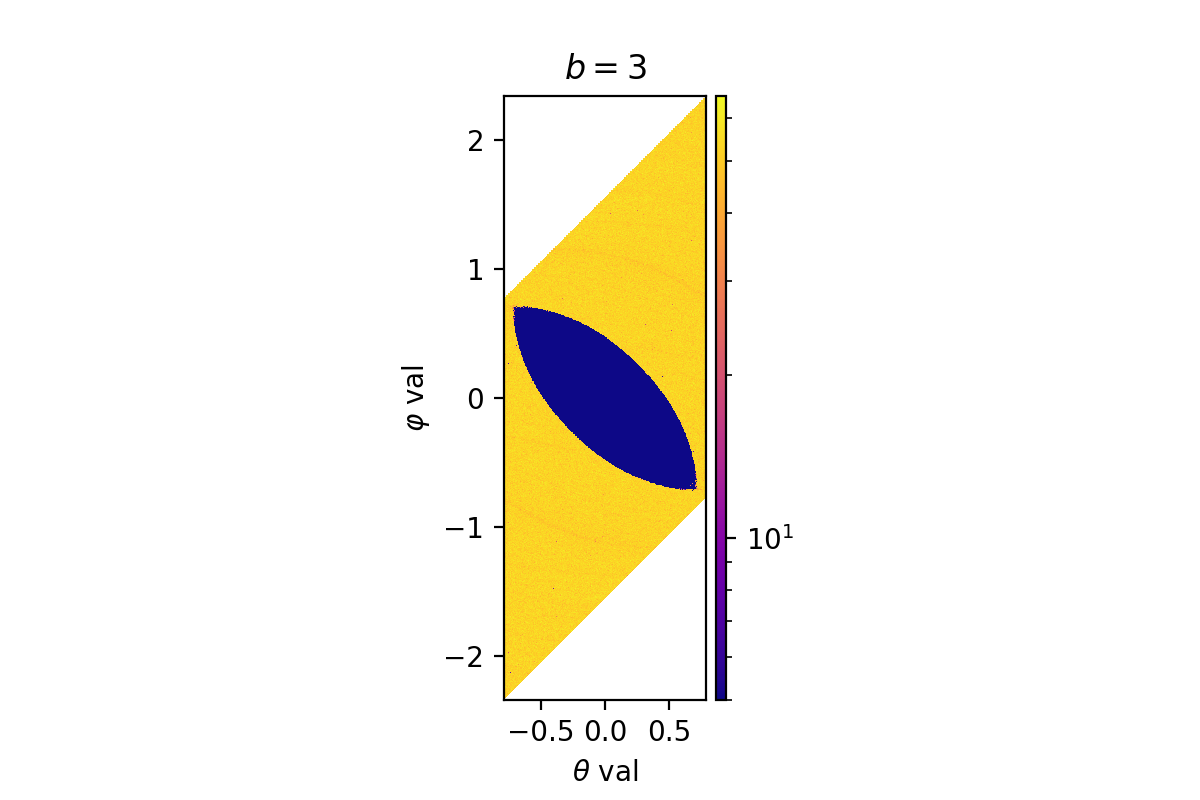
\includegraphics[width=\textwidth, trim={5cm 0cm 4cm 0cm}, clip]{LZ_th_ph_b_3_sweep.png}
\caption{}
\label{subfig:LZpoincaresectionb3}
\end{subfigure}
%
\begin{subfigure}[h]{0.49\textwidth}
\centering
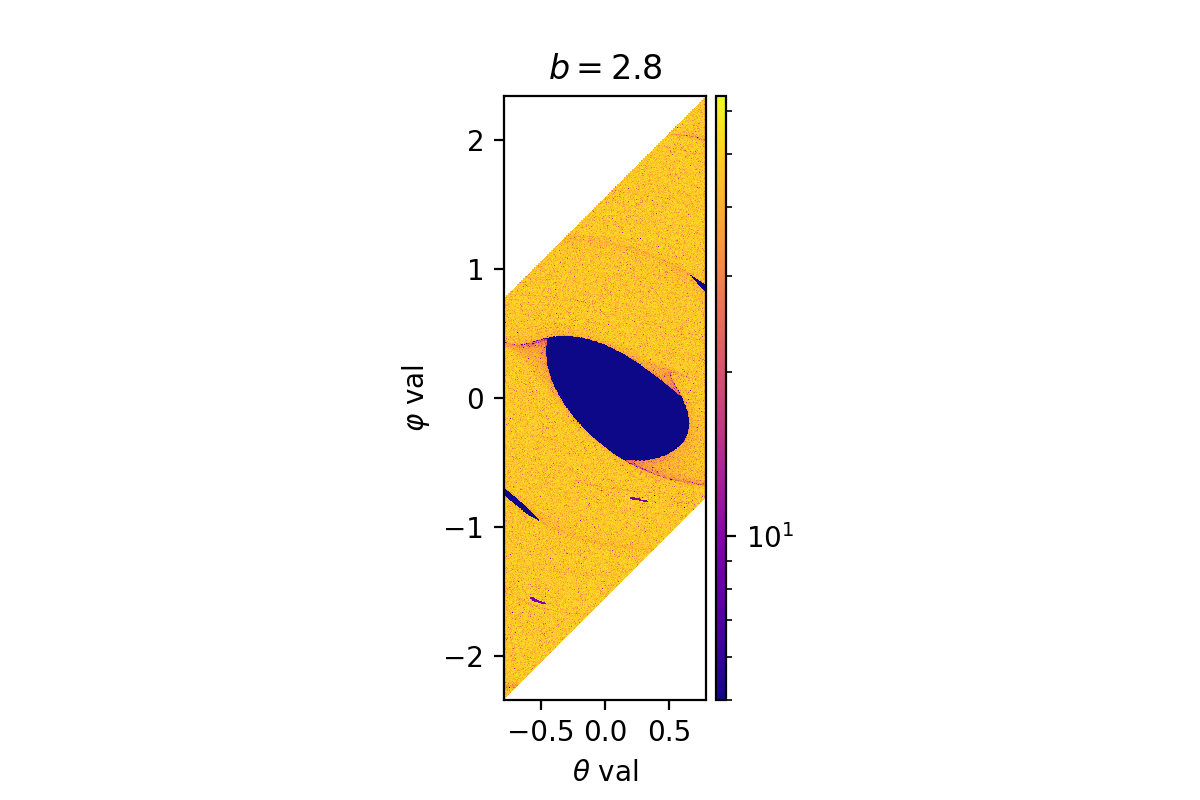
\includegraphics[width=\textwidth, trim={5cm 0cm 4cm 0cm}, clip]{LZ_th_ph_b_2.8_sweep.png}
\caption{}
\label{subfig:LZpoincaresectionb2.8}
\end{subfigure}
\caption{LZC plot of a few Poincar\'e sections}
\label{fig:LZpoincare1}
\end{figure}

In \cref{subfig:LZpoincaresectionb3}, we again focus on $b=3$, which has the periodic trajectory \cref{subfig:penandpaperorbits1}. The dynamics appears to be simple, there is a large region of quasi-periodic trajectories around $(\theta,\varphi)=(0,0)$, and the rest is uniformly high LZC. In \cref{subfig:LZpoincaresectionb2.8}, we perturb $b=2.8$, the stable region from \ref{subfig:LZpoincaresectionb3} changed shape, it is smaller, and there are now more noticeable artifacts along the boundary. Besides that, we see new stable regions: one larger, and two small. The two small ones likely belong to the same quasi-periodic trajectory, while the larger region belongs to its own. Looking back at \cref{subfig:strangesquare}, since there we had $b=2.805$, we see indicated a periodic trajectory along the bottom edge of the Poincar\'e section. Here, we expect a similar trajectory, perhaps slightly perturbed. It's interesting to note that in \cref{subfig:LZpoincaresectionb3} we see faint streaks in the same spots where there are stable regions in \cref{subfig:LZpoincaresectionb2.8}. We conjecture that the patterns and streaks in the noise suggest a nearby bifurcation.

\begin{figure}[!th]
\centering
\begin{subfigure}[h]{0.49\textwidth}
\centering
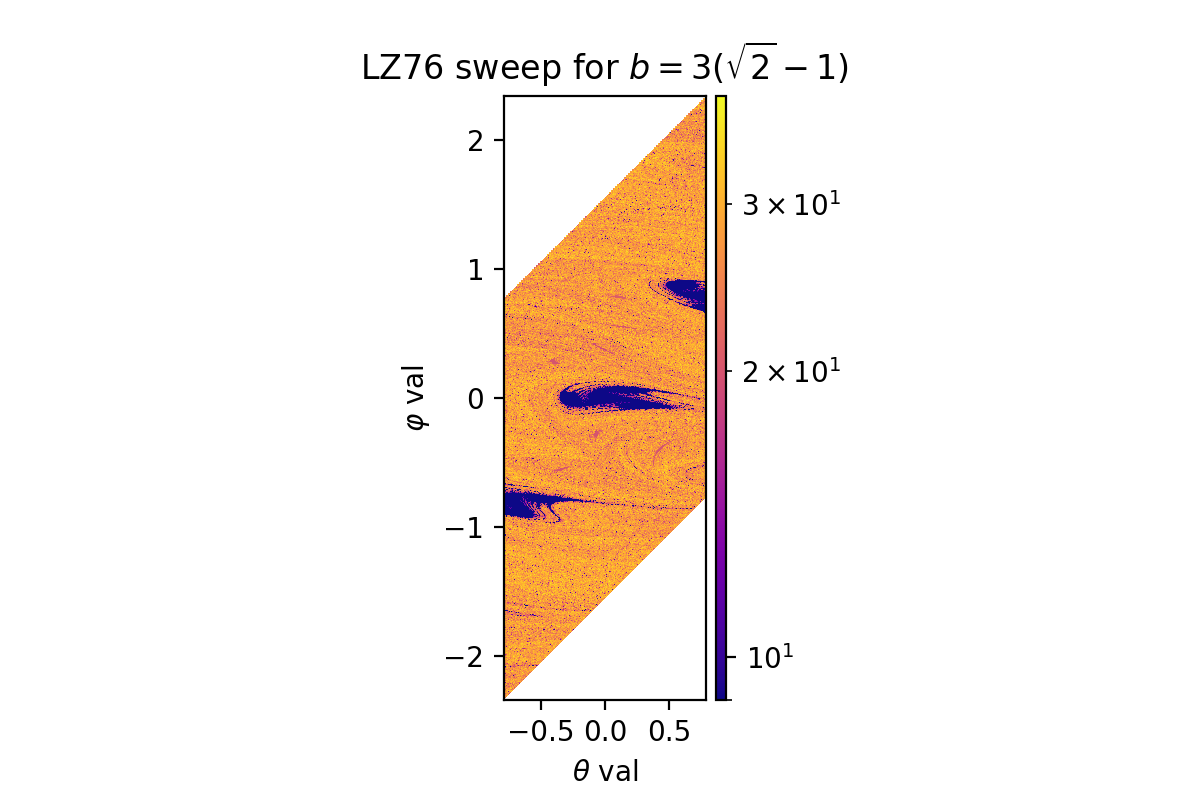
\includegraphics[width=\textwidth, trim={5cm 0cm 4cm 0cm}, clip]{LZ_th_ph_b_3sqrt2-1_sweep.png}
\caption{}
\label{subfig:LZpoincaresectionb1242}
\end{subfigure}
%
\begin{subfigure}[h]{0.49\textwidth}
\centering
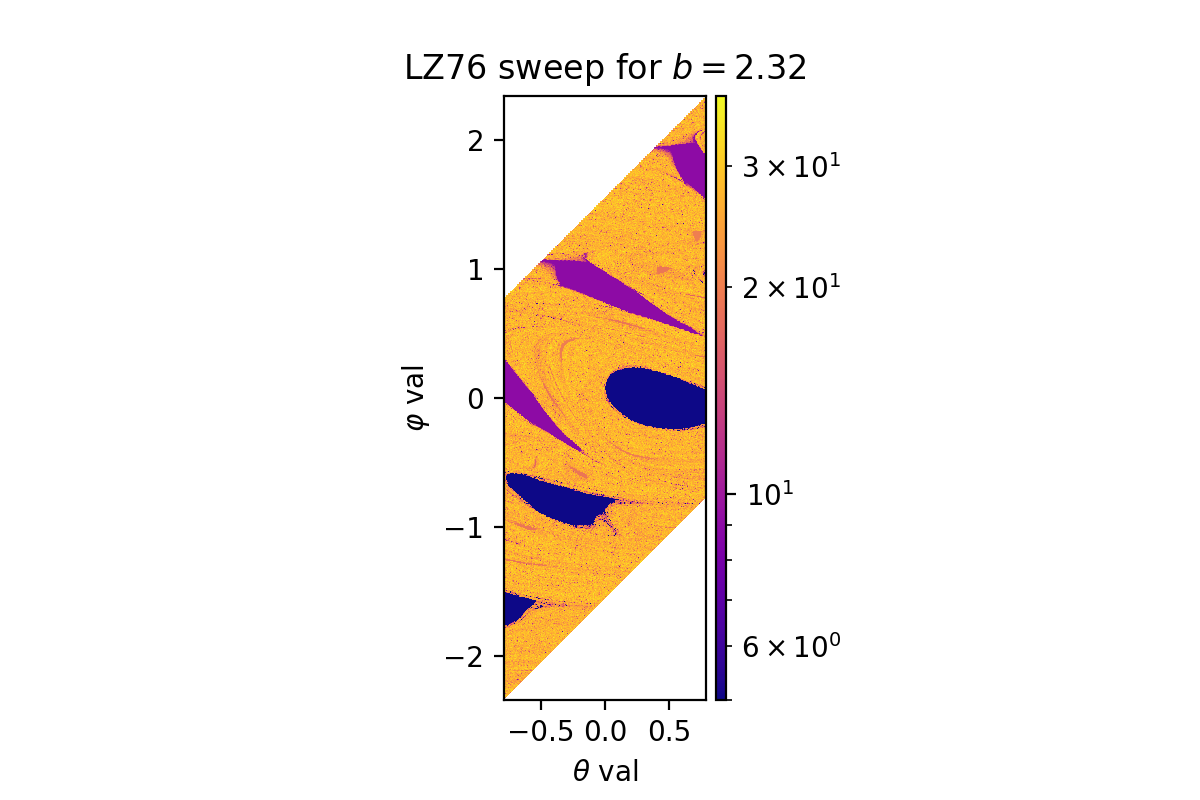
\includegraphics[width=\textwidth, trim={5cm 0cm 4cm 0cm}, clip]{LZ_th_ph_b_2_32_sweep.png}
\caption{}
\label{subfig:LZpoincaresectionb232}
\end{subfigure}
\caption{Another  LZC plot of a few Poincar\'e sections}
\label{fig:LZpoincare2}
\end{figure}
In \cref{subfig:LZpoincaresectionb1242} we plot the same data except $b\approx3(\sqrt2-1)$, corresponding to \cref{subfig:penandpaperorbits3}. The size of the blue regions is about the same, so there should relate to the same quasi-periodic orbit. What's different in this case is the pronounced teardrop with fractal-like structure. If we were to iterate deeper, it looks like the fractal branches would connect to make 4 disjoint blue blobs. Around the main big region, we see smaller red specks, suggesting another quasi-periodic trajectory that we didn't expect before.

In \cref{subfig:LZpoincaresectionb232}, $b=2.32$, the kind of quasi-periodicity here should be similar to \ref{subfig:lopsidedhexagon}, \ref{subfig:ornamet1}, and \ref{subfig:star2}. It's plausible there are 3 different quasi-periodic regions here, since you can separate the blobs easily into three sets: blue along the bottom, purple along the top, and small red in between.

